%%%%%%%%%%%%%%%%% PREAMBLE %%%%%%%%%%%%%%%%%%%%%%%%%%%%
%Change the font size of your document - 10pt, 12.1pt, etc.
\documentclass[letterpaper,12pt,oneside]{article}
\usepackage[utf8]{inputenc}
\usepackage{setspace}
\usepackage{hyperref}
\usepackage{graphicx}
\usepackage{bibentry}
\usepackage[left=1.02in, right=1.02in, bottom=1.15in, top=0.85in]{geometry}
\usepackage[pages=all]{background}
\usepackage{transparent}

%Changes the page numbers - {arabic}=arabic numerals, {gobble}=no page numbers, {roman}=Roman numerals
\pagenumbering{gobble}
%%%%%%%%%%%%%%%%% END OF PREAMBLE %%%%%%%%%%%%%%%%%%%%%

\backgroundsetup{
scale=1,
color=black,
opacity=0.16,
angle=0,
contents={%
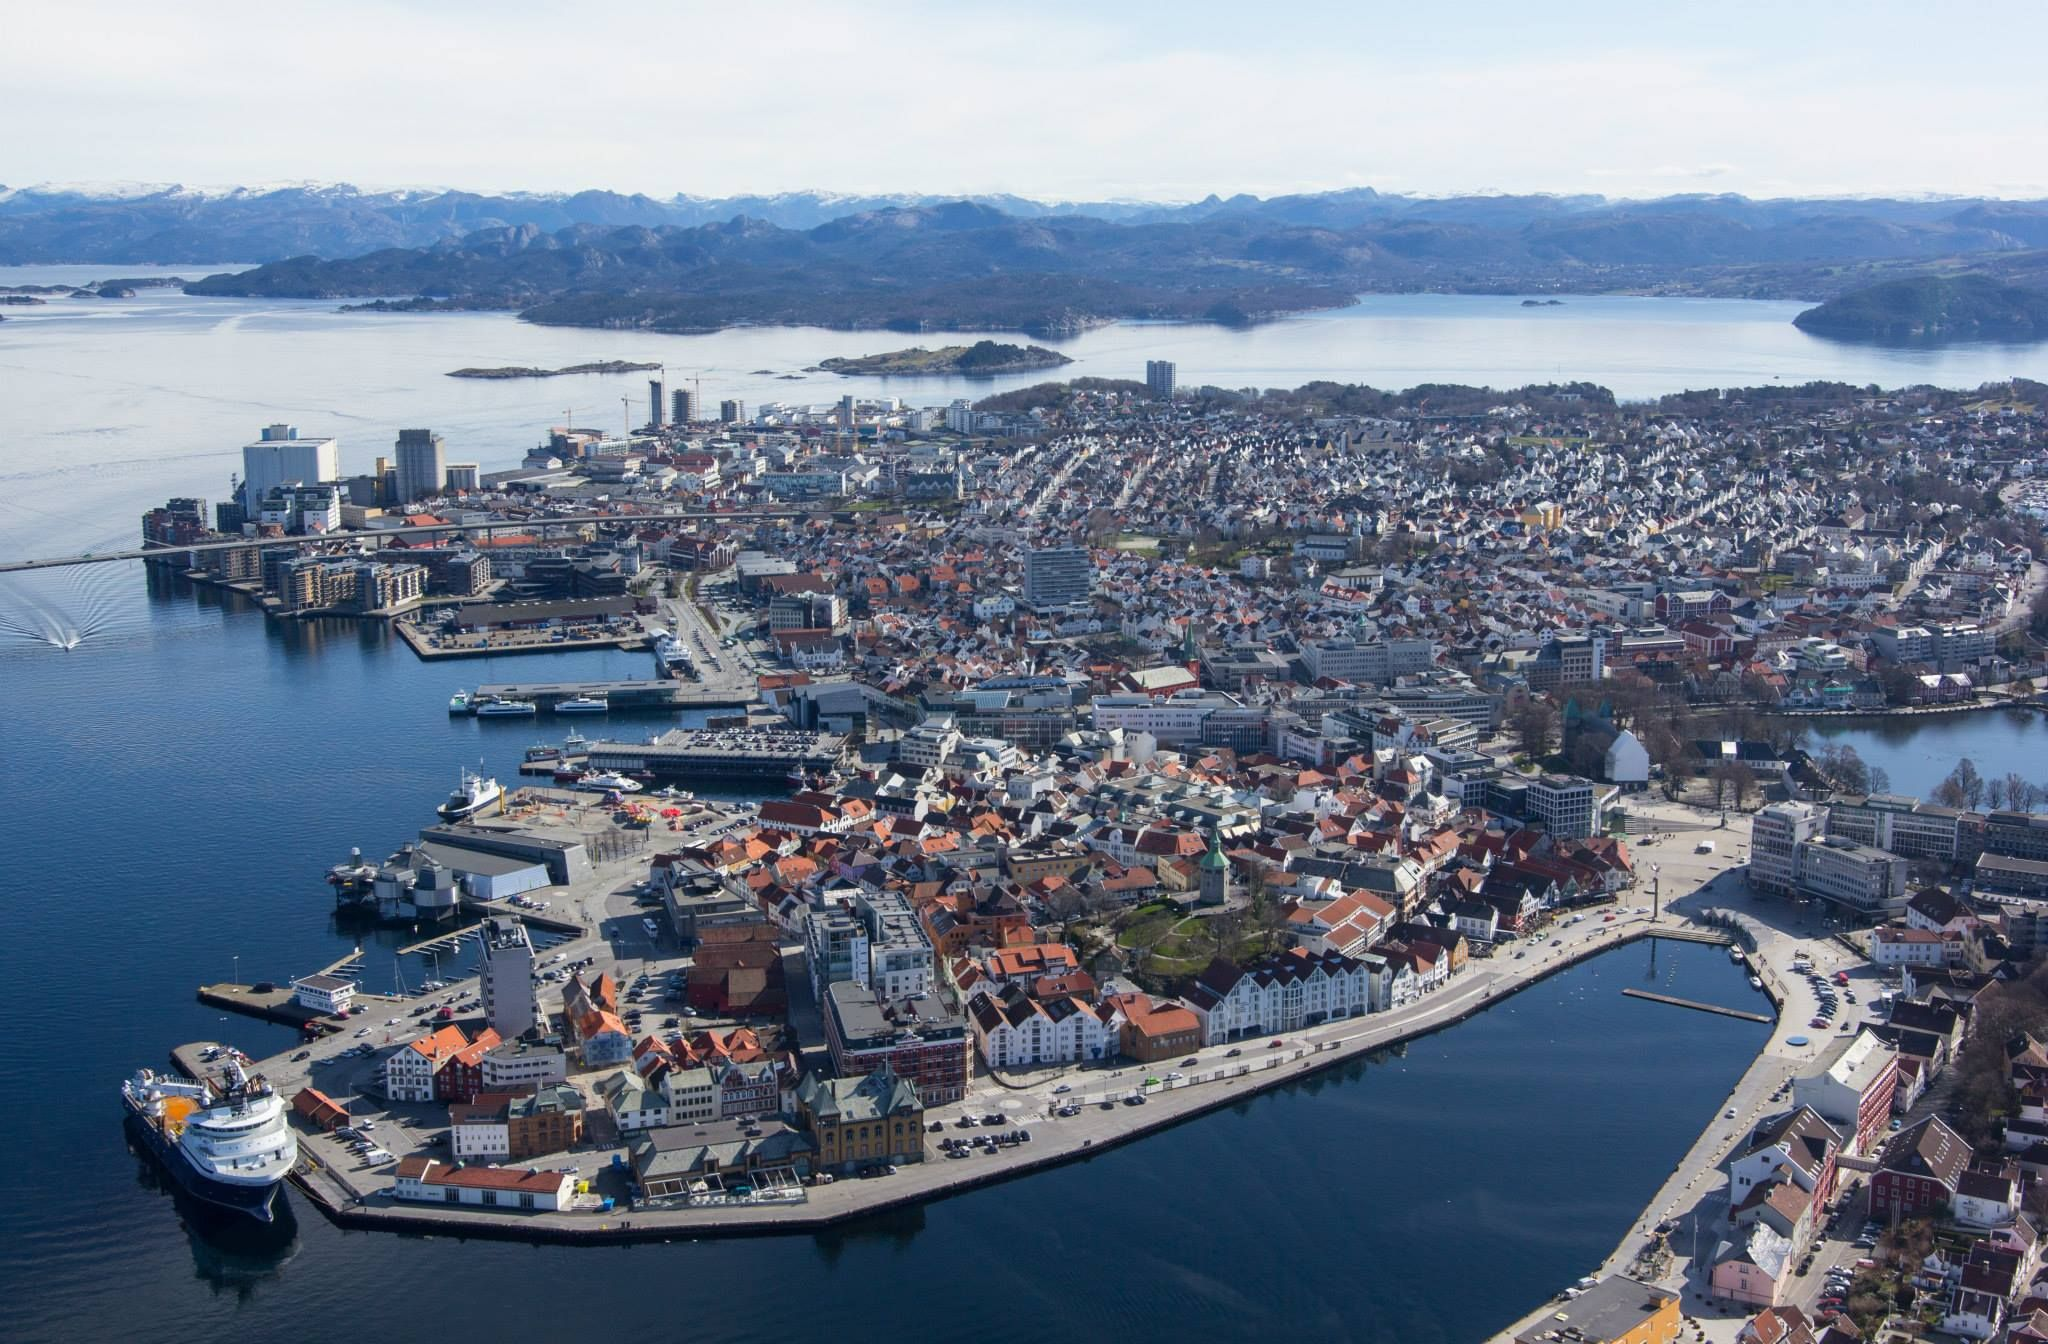
\includegraphics[width=\paperwidth,height=\paperheight]{stv.jpg}
}%
}
\begin{document}
\begin{flushright}
\transparent{0.99}
\includegraphics[scale=0.5]{uis_logo.jpeg} 
\end{flushright}


\vspace{-8.3em}
\begin{flushleft}
\Large\textit{\bf  --- Course Overview ------------------- \\
MOD550: Fundaments of Machine learning \\ for and with
engineering applications   \\   }
\end{flushleft}

---------------------------------------------------------------------------------------

\vspace{1.5em}

\begin{flushleft}
\textit{"The goal is to turn data into information, and information into insight"} \\
Carly Fiorina, Former CEO of HP

\end{flushleft}

\section*{Introduction}
Machine learning has recently emerged as one of the most promising resources for engineers, offering a set of powerful approaches to tackle complex engineering challenges. By employing various statistical techniques in learning algorithms, machine learning enables the development of predictive models, optimization strategies, and decision support systems that can enhance the design, analysis, and control of engineered systems. This technology empowers engineers to extract meaningful insights from vast datasets, automate repetitive tasks, and improve the efficiency, reliability, and performance of engineering processes. Its applications span diverse domains, from mechanical and chemical engineering to geo, material science, etc. making machine learning an indispensable resource for modern computational engineers for physics based and data-driven solutions to real-world problems.

Most undergraduates in engineering and science fields have little exposure to data methods, while most computer scientists and statisticians have little exposure to dynamical system control. Our goal is to provide an entry point and interface for both these groups of students. 

\section*{Learning outcomes}

\item  Understanding of engineering data sources and consequent data properties, statistics, and probability distributions (from feature engineering to digital twins).
\item  Understanding of data analysis/machine learning approaches outcomes, method sensitivity and their applications (e.g. molecular modeling, flow simulation, geoscience).
\item Understanding of deep learning principles and its advantages/limitations in engineering applications. 
\item Predictive modeling (using simulation, machine learning, and Generative AI such as ChatGPT).
\item Multivariate data analysis including principal component, cluster, and discriminant analysis
\item Applying machine learning techniques (e.g., random forest, gradient boosting machine, support
vector regression, and kriging model) for predictive modeling.
\item Understand sensitivity analysis and the information it provides.
\item Visualization and reporting to provide input for a decision by communicating information to
decision-makers.

\end{itemize}
\section*{Skills}
\begin{itemize}

  \item  Data handling, data wrenching and feature engineering.
 \item   Can develop data driven models of physical systems for chemical and mechanical engineering, material science and geology. 

  \item  Test data driven models against physical models and experimental data.
 \item   Apply appropriate statistical methods to obtain better insights.
 \item   Develop own programs written in Python and develop wrappers for open machine learning repositories. 
     
\end{itemize}


\section*{General qualifications:}

\begin{itemize}
\item Can identify engineering problems, develop hypotheses, and apply mathematical models and data driven solutions.
\item Can structure different statistical models in a wide range of engineering applications.
\item Can connect engineers and data science solutions -both to specialists and to the general public.

\end{itemize}



\section*{Content}


The focus of this course is the basic knowledge and related assumptions involved in applying statistics and machine learning in spatial and/or temporal contexts. The emphasis is on providing students with knowledge of the fundamentals of statistics and machine learning most relevant for spatial or temporal data. 

The core of the course is data analysis with a clear focus on engineering applications. Data sources, their quality, and consistency will be discussed to guide the selection of suitable spatial and temporal models. Simulation techniques are introduced as a means of modeling heterogeneity and uncertainty. Machine learning techniques, such as regression modeling and analysis and multivariate data analysis, will be introduced and applied. Python and other programming tools will be used for modeling, preparing spatial and temporal data, scripting statistical workflows, and constructing visualizations to communicate model outputs and analysis results. 

The primary purpose of modeling is to generate decision insight. That is the criteria to assert the 'usefulness’ of a model and along which its interpretability, resolution and outcome accuracy will be evaluated in a set of given tasks. 




\section*{Course Staff}



Instructors:

Enrico Riccardi,
Email: enrico.riccardi@uis.no
Office: E-301B

Reidar B Bratvold,
Email: reidar.bratvold@uis.no
Home page: www.reidar-bratvold.com
Office: E-396 

Remus Gabriel Hanea 
Email: rhane@equinor.com 


\section*{Class Delivery}


We will meet physically in the lecture room 6 hours per week most of the semester. A
great deal of the learning and value of this course comes from in-class discussions;
therefore, attending lectures regularly and keeping up with the readings and assignments
is essential to ensure a rewarding learning experience (as well as a good grade).
The lectures will include some interactive computer work (not recorded). Independent readings
throughout the semester are expected.
The sessions will also include interactive Python implementations and coding. You are
expected to have Python installed (more information below) on your computers.
The interactive sessions will expand upon and add details to the curriculum covered in
the lectures. In these sessions we will show examples of how to use and implement
models and analyses discussed, illustrate how to solve problems, show solutions to
assignments and respond to any questions you may have on the curriculum. Jupyter
Notebooks and solutions to assignments will not be made available on
Canvas.
Compulsory problem sets (4-6) will be assigned throughout the semester. You must pass
these to be allowed to take the exam. These assignments provide an excellent opportunity to practice
questions and problems of the type that will be given on the final test. Solutions to these
exercises will not be handed out but will be discussed in the classroom. Exceptions might be made \textbf{only for exceptional cases} where the students have mobility limitations and the instructors are informed \textbf{well in advance}.


\section*{First day of lectures}

Tuesday 14th January


\section*{Class Times and Locations}
  

\begin{center}
\begin{tabular}{ c c c c c }

Course week & Calendar Week & day 1 & day 2 & Lecturer \\
1 &  3 & 14.1 (2hrs) & 16.1 (4hrs) & Enrico \\
2 &  4 & 21.1 (3hrs) & 23.1 (3hrs) & Enrico \\
3 &  5 & 28.1 (3hrs) & 30.1 (3hrs) & Enrico \\
4 &  6 &  4.2 (3hrs) &  6.2 (3hrs) & Enrico \\

5 &  7 & & 13.2 (6hrs) & Remus \\

6 &  8 & 18.2 (3hrs) & 20.2 (3hrs) & Reidar \\
7 &  9 & 25.2 (3hrs) & 27.2 (3hrs) & Reidar \\
8 &  10 &  4.3 (3hrs) & 6.3 (3hrs) & Reidar \\
9 &  11 & 11.3 (3hrs) & 13.3 (3hrs) & Reidar  \\

10 &  14 & &  3.4 (6hrs) & Remus \\
11 &  15 & & 10.4 (6hrs) & Remus \\
12 &  16 & & 24.4 (6hrs) & Remus 

\end{tabular}
\end{center}


3 hrs lecures (Enrico \& Reidar):  

\begin{center}
\begin{tabular}{ c c c  }
Day &  Room &  Time \\
Tuesday & KE A-202 & 13:15 – 16:00 \\
Thursday & KE A-203 & 13:15 – 16:00

\end{tabular}
\end{center}

6 hrs lecures (Remus): 

\begin{center}
\begin{tabular}{ c c c }
Day &  Room &  Time \\
Thursday & KE A-203 & 12:15 – 18:00

\end{tabular}
\end{center}


\section*{Assumed Knowledge}
 
BSc in Engineering/Economics/Mathematics/Geoscience. Basic understanding of coding.

\section*{Assessment}

The grade for the course will be based on folder evaluation (mappe-evaluering) as follows:
Weight
Final exam (digital on campus) 1/1
A portfolio containing 4-6 assignments needs to be approved to take the final exam. The students
may cooperate on the assignments but must hand in their individual assignments which should
not be copies of other students’ assignments.
In addition to being required for access to the exam, these assignments provide an excellent
opportunity to practice questions and problems of the type that will be given on the exam.


\section*{Modeling and Programming}

Many of the assignments will require the development of models by using mathematical
programming. We will use Python for this. We will provide Python tutorials on Canvas and show
live coding during interactive sessions. However, you should also use the web actively for questions
on Python programming.

 
 \vspace{4em}
\section*{Looking forward to meet you}

\end{document}


